\section{Verification}

%===============================================================================
% NEW SLIDE
%===============================================================================
\begin{frame}
\frametitle{Verification: Finding The Unknown Unknowns}
\begin{block}{Solution Verification}
Estimating Numerical Error:
\begin{itemize}
\item Discretization Error
\item Iterative Error
\item Round-off Error
\end{itemize}
These errors cannot be avoided, but can be quantified.
\end{block}
\begin{block}{Code Verification}
\begin{itemize}
\item Software bugs
\item Numerical algorithm weaknesses
\item Model implementation mistakes
\end{itemize}
Codes cannot be proven error-free, but can be proven to
have errors.  So we take every opportunity to do the latter...

\end{block}

\end{frame}


\subsection{Designing for Reuse}

%===============================================================================
% NEW SLIDE
%===============================================================================
\begin{frame}
\frametitle{Code Reuse, Modularity}
\begin{columns}
\begin{column}{.5\textwidth}

\begin{itemize}
\item Errors are easier to find in smaller problems

\item Extend existing capabilities where possible
\end{itemize}

\begin{center}
\includegraphics[width=.5\textwidth]{modular_fem}
\end{center}

\end{column}

\begin{column}{.5\textwidth}
\begin{center}
\includegraphics[width=.6\textwidth]{fins_modules}
\end{center}

\begin{itemize}
\item More eyes == more testing

\item Code you don't write is code you don't write bugs in
\end{itemize}

\end{column}
\end{columns}

\end{frame}


%===============================================================================
\begin{frame}[fragile]
\frametitle{Assertions}

\vfill

``When in trouble when in doubt, run in circles scream and shout.''\\
- old Army War College football team slogan

\pause
\vfill

\begin{block}{\texttt{assert(!in\_trouble());}}

\begin{verbatim}
#if IN\_DOUBT {           // not an optimized build
  if (in\_trouble()) {    // expected condition fails
    run\_in\_circles();   // Output debug info
    scream\_and\_shout(); // Throw exception
  }
#endif
\end{verbatim}

\end{block}

\end{frame}



%===============================================================================
% NEW SLIDE
%===============================================================================
\begin{frame}
\frametitle{High-level Assertions}
\begin{block}{{\texttt{libmesh\_assert()}, \PETSc} debug mode}
\begin{itemize}
\item Active only in ``debug'' runs: `METHOD=dbg` and `METHOD=devel`
\item Function preconditions
\begin{itemize}
\item Are function arguments all valid?
\end{itemize}
\item Function postconditions
\begin{itemize}
\item Does function result satisfy requirements?
\end{itemize}
\item Approx. 7000 assertions in \libMesh{}, \texttt{TIMPI}, and
  \texttt{MetaPhysicL}
\end{itemize}
\end{block}

 \begin{block}{\libMesh{} Assertions}
Standard \texttt{assert()} prints failed assertion, file/line numbers

\texttt{libmesh\_assert()} adds:
\begin{itemize}
\item Data from specialized assertions
\item Per-rank stack trace files, line numbers
\item \cpp{} exception thrown
\end{itemize}
\end{block}

\end{frame}

%===============================================================================
% NEW SLIDE
%===============================================================================
\begin{frame}[fragile]
\frametitle{High-level Assertions Examples}
{\footnotesize
\begin{verbatim}
libmesh_assert_less(c, _variables.size());
libmesh_assert_less(s, elem->n_sides());
libmesh_assert((ig >= Ug.first_local_index()) &&
               (ig < Ug.last_local_index()));
libmesh_assert_equal_to(requested_ids[p].size(),
                        ghost_objects_from_proc[p]);
libmesh_assert_not_equal_to(obj_procid,
                            DofObject::invalid_processor_id);
MeshTools::libmesh_assert_valid_node_procids(mesh);
libmesh_assert(neigh->has_children());
libmesh_assert(this->closed());
libmesh_assert(this->initialized());
libmesh_assert(mesh.is_prepared());
libmesh_assert(error_type == H1_SEMINORM ||
               error_type == W1_INF_SEMINORM)
libmesh_assert(number_h_refinements > 0 ||
               number_p_refinements > 0);
\end{verbatim}
}
\end{frame}

%===============================================================================
% NEW SLIDE
%===============================================================================
\begin{frame}
\frametitle{Lower-level Assertions}
  \begin{block}{Low-level verification options}
\begin{itemize}
\item \texttt{configure --enable-glibcxx-debugging}
\begin{itemize}
\item Runtime bounds checking of standard \texttt{vector},
iterator use
\item Runtime consistency checking of ordered \texttt{set},
  \texttt{map}, etc.
\end{itemize}
\item UBSAN, ASAN in gcc, clang
\item Valgrind memcheck, helgrind
\item Bounds checking is too expensive to do by default
\item Out Of Bounds errors are Undefined Behavior
\begin{itemize}
  \item Corrupt data, not just segfaults!
\end{itemize}
\end{itemize}
\end{block}

\end{frame}


%===============================================================================
% NEW SLIDE
%===============================================================================
\begin{frame}
\frametitle{Unit Tests}
\begin{block}{Testing One Object At A Time}
\begin{itemize}
\item Reusable modules interact with all other code through a limited
API
\item That API can be tested directly outside of application code
\item Test one method at a time, isolate problems locally
\item 4000-5000 unit tests are in \libMesh{}
\begin{itemize}
  \item 673 abstract unit test codes, plus many runtime instantiations
    for subclasses: Elem, FE, NumericVector, etc.
  \item More test coverage when considering compile-time options
\end{itemize}
\end{itemize}
\end{block}

\pause

\begin{block}{Tests are useful {\bf only when run}!}
\begin{itemize}
\item Regression, example, application tests had more coverage
\item Unit tests became useful only when added to CI
\item Most useful: Test-driven development
\begin{itemize}
    \item Write tests first
    \item Write code to fit
\end{itemize}
\end{itemize}
\end{block}
\end{frame}


%===============================================================================
% NEW SLIDE
%===============================================================================
\begin{frame}[fragile]
\frametitle{Unit Tests Example}
{\footnotesize
\begin{verbatim}
#include <quadrature.h>

class QuadratureTest : public CppUnit::TestCase {
public:
  CPPUNIT_TEST_SUITE( QuadratureTest );
  CPPUNIT_TEST( test3DWeights<FIFTH> );  // etc.

  template <Order order>
  void test3DWeights ()
  {
    auto qrule = QBase::build(QGAUSS, 3, order);
    qrule->init (TET10);
    sum = 0;
    for (auto qp : make_range(qrule->n_points()))
      sum += qrule->w(qp);
    CPPUNIT_ASSERT_DOUBLES_EQUAL(1/Real(6), sum ,
                                 TOLERANCE*TOLERANCE);
  }
};
\end{verbatim}
}
\end{frame}




\subsection{Library Verification}

%===============================================================================
\begin{frame}
\frametitle{Verification Benchmark Problems}
\begin{block}{Choosing Test Problems}

Capitalize on anything you know a priori:

\begin{itemize}
\item Known solutions
\begin{itemize}
\item Exact solution to discretized problem
\item Limit solution of continuous problem
\item Known quantities of interest
\end{itemize}
\item Manufactured solutions
\item Known asymptotic convergence rates
\item {\bf Known residuals}
\item ``Gold solutions'' to catch regressions
\end{itemize}
\end{block}
\end{frame}

%===============================================================================
% NEW SLIDE
%===============================================================================
\begin{frame}
\frametitle{Known Solutions, Functionals}
\begin{block}{Examples}
\begin{itemize}
\item Incompressible flow around a cusp
\item Wetting angle in Laplace-Young surface tension
\end{itemize}
\end{block}

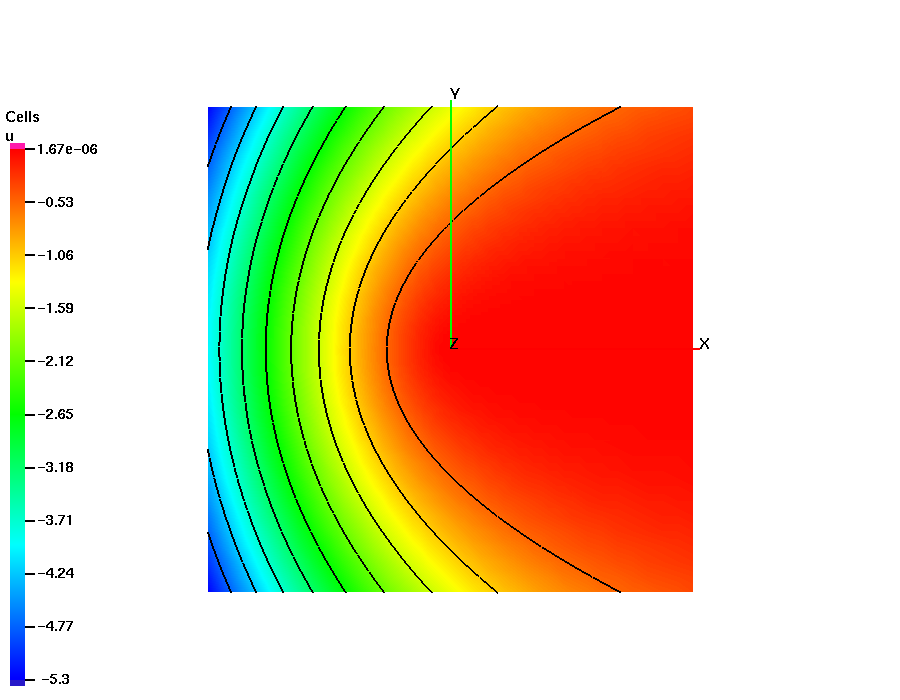
\includegraphics[width=.3\textwidth]{cuspflow}
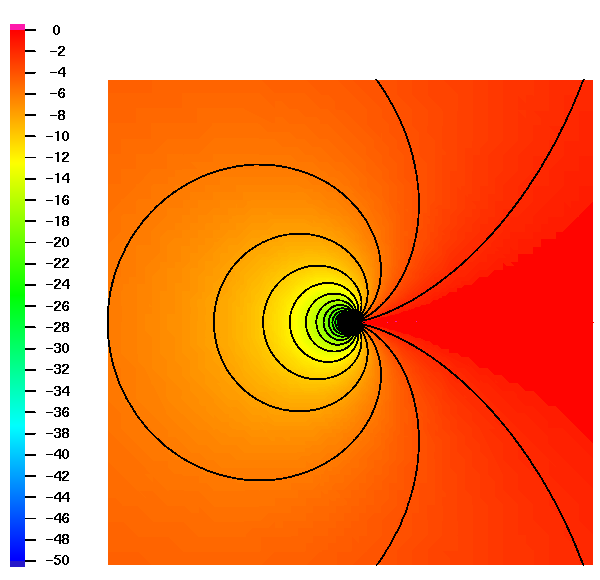
\includegraphics[width=.3\textwidth]{cuspvorticity}
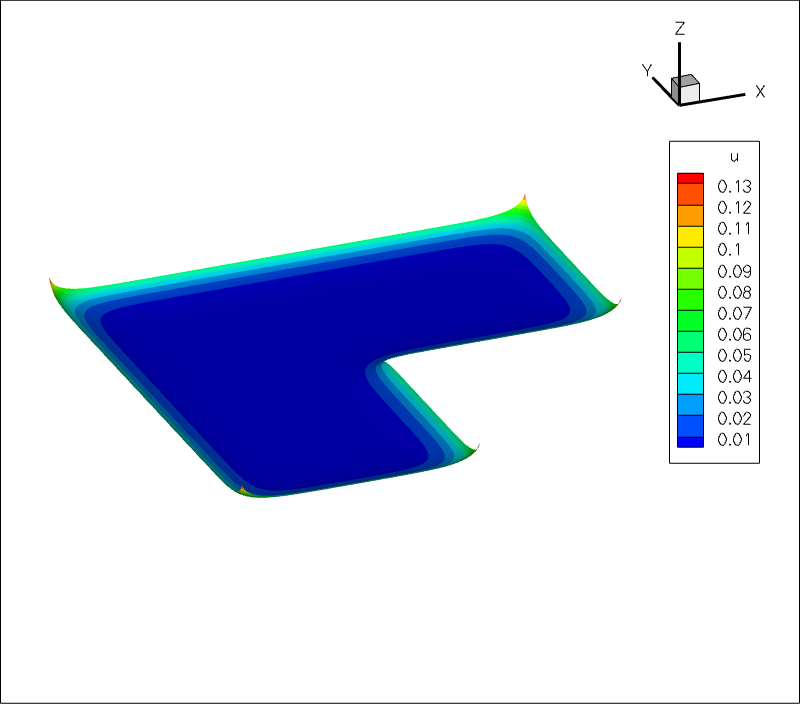
\includegraphics[width=.3\textwidth]{ly_over_3d}

\end{frame}

%===============================================================================
% NEW SLIDE
%===============================================================================
\begin{frame}
\frametitle{Manufactured Solutions}
\begin{block}{Any Solution for Any Equation}
\begin{itemize}
\item Real Physics: $\V{R}(\V{u}) = 0$ for $\V{u} = \V{u}^r$
\item Choose manufactured solution $\V{u}^m$
\item Desired Physics: $\V{R}^m(\V{u}) = 0$ for $\V{u} = \V{u}^m$
\item Construct $\V{R}^m(\V{u}) \equiv \V{R}(\V{u}) - \V{R}(\V{u}^m)$
\end{itemize}
\end{block}

\end{frame}

%===============================================================================
% NEW SLIDE
%===============================================================================
\begin{frame}
\frametitle{Manufactured Solution Example}
\begin{columns}
\begin{column}{.7\textwidth}
\begin{block}{Convection-Diffusion Problem with Adjoints}
Residual equation:
\begin{equation*}
\V{R}(\V{u}) = \nabla \cdot \alpha \nabla \V{u} + \beta \vec{e}_x \cdot \nabla
\V{u} + \V{f} = 0
\end{equation*}
Manufactured solution:
\begin{equation*}
\V{u} \equiv 4(1 - e^{-\alpha x} - (1 - e^{-\alpha})x)y(1-y)
\end{equation*}
\begin{itemize}
\item Homogeneous Dirichlet boundary
\item $\alpha$ controls flux strength, layer
\item Choose any convection strength $\beta$, solve for $\V{f}$
\item $\beta = 0$ gives simple series adjoint solutions
\end{itemize}
\end{block}
\end{column}
\begin{column}{.3\textwidth}
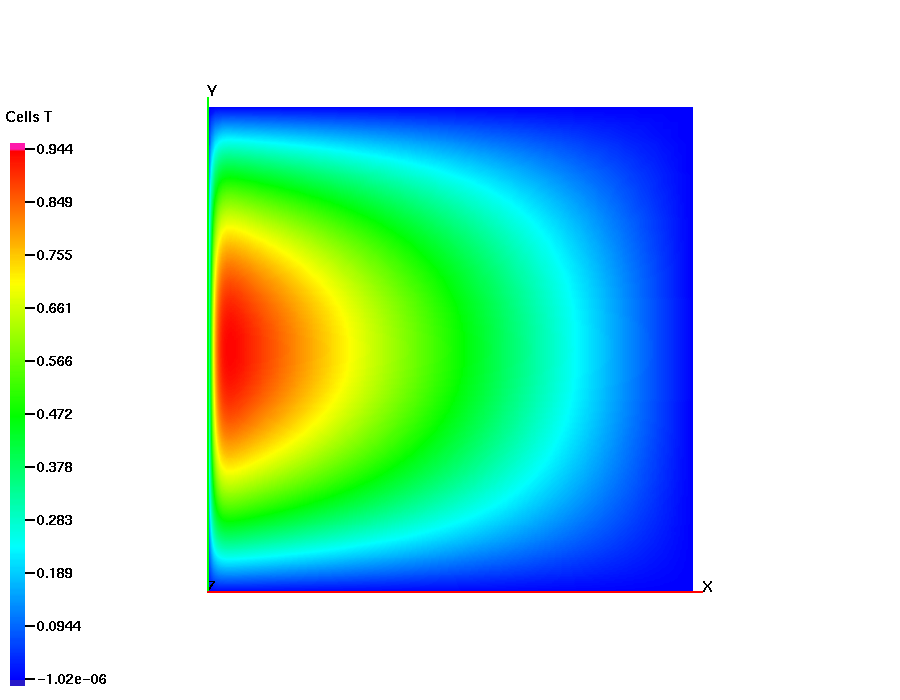
\includegraphics[width=\textwidth]{layer}

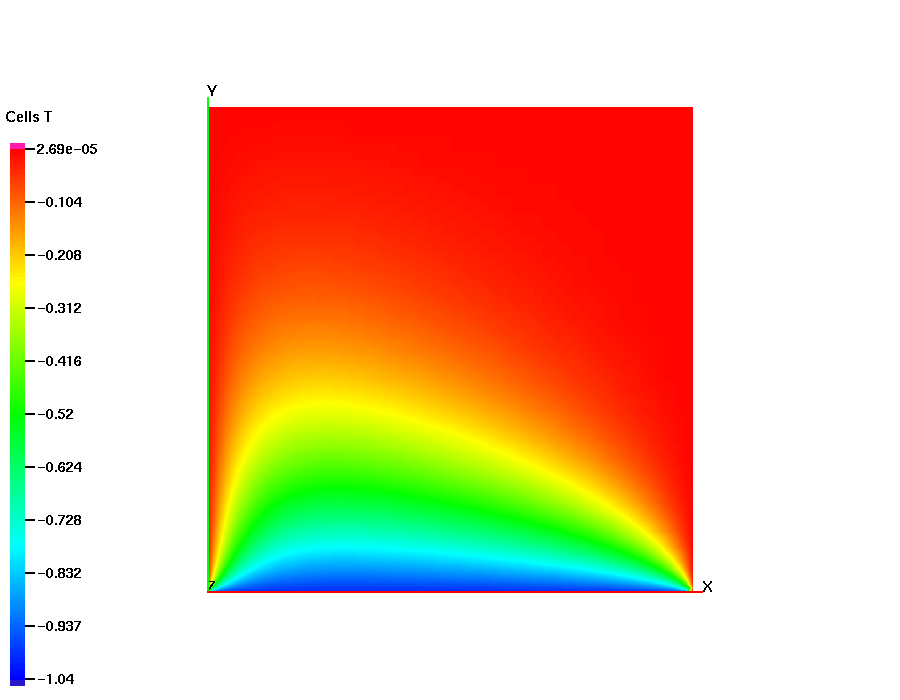
\includegraphics[width=\textwidth]{adjoint_conv}

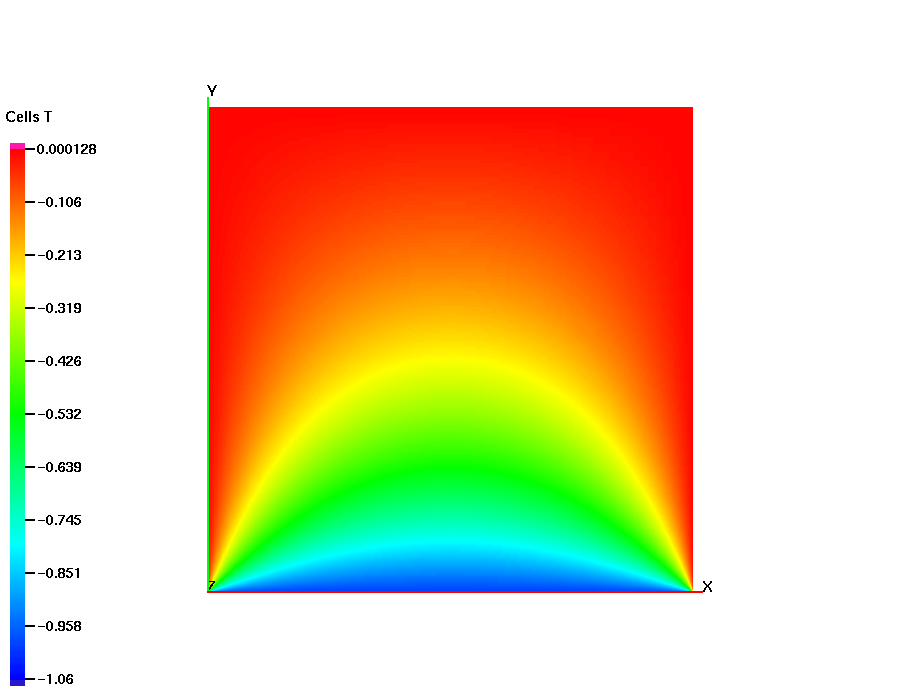
\includegraphics[width=\textwidth]{adjoint}
\end{column}
\end{columns}

\end{frame}

%===============================================================================
\begin{frame}
\frametitle{Manufactured Solution Example}
\begin{columns}
\begin{column}{.7\textwidth}
\begin{block}{Goal-Oriented Refinement}
\begin{itemize}
\item Superconvergence on some grids
\item Convergence ``plateaus'' found in multiple refinement strategies
\item \texttt{UniformRefinementEstimator} required new code to
solve for adjoint solution errors
\item \texttt{PatchRecoveryErrorEstimator} required new seminorm
integration ($H^1$/$L_2$/mixed vs. $W^{1,\inf}$) to give compatible error subestimates
\end{itemize}
\end{block}
\end{column}
\begin{column}{.3\textwidth}
\begin{center}
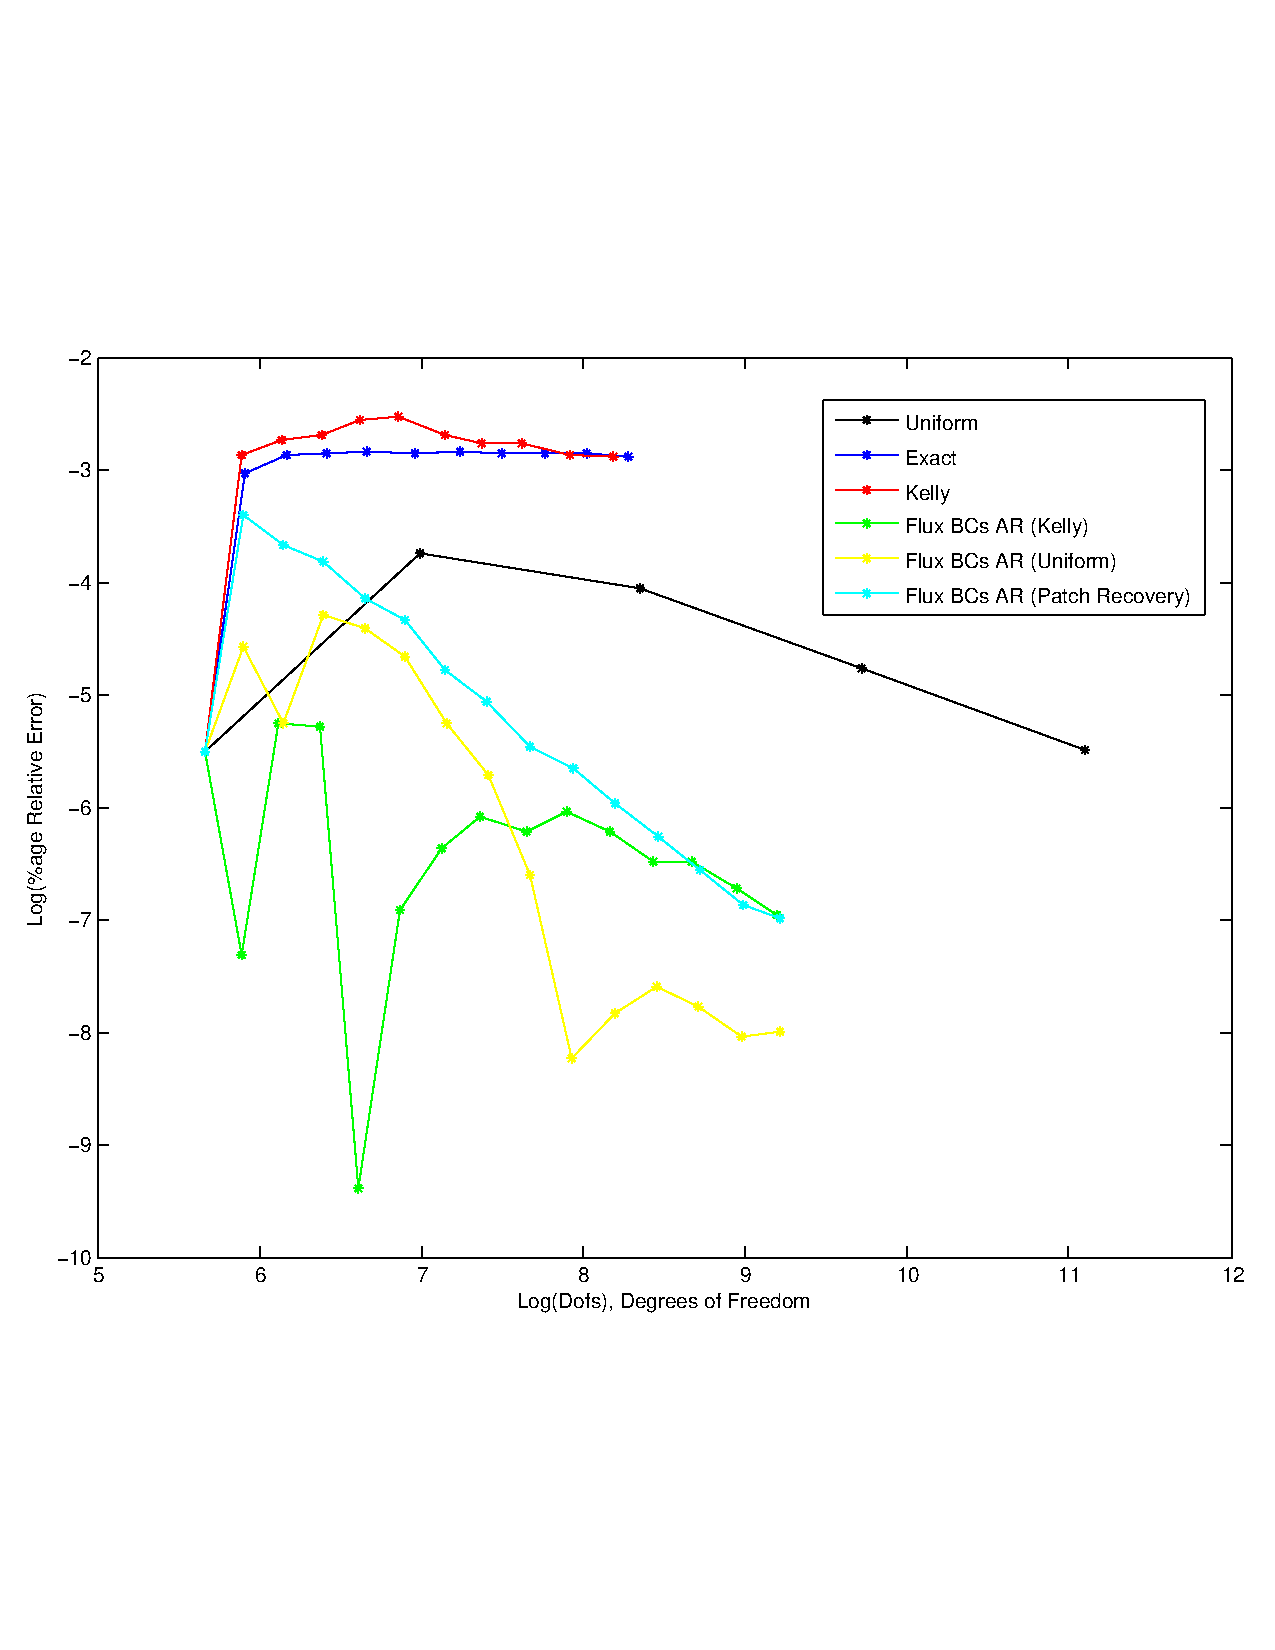
\includegraphics[width=\textwidth]{qoi_convergence}
\end{center}
\end{column}
\end{columns}

\begin{center}
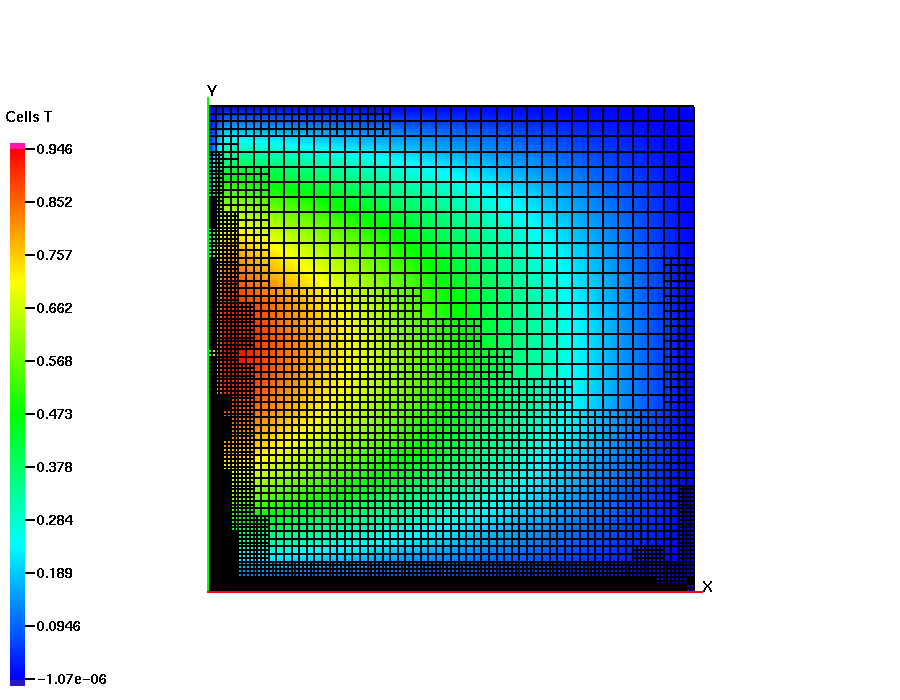
\includegraphics[width=.3\textwidth]{adjoint_grid1}
\;\;\;\;
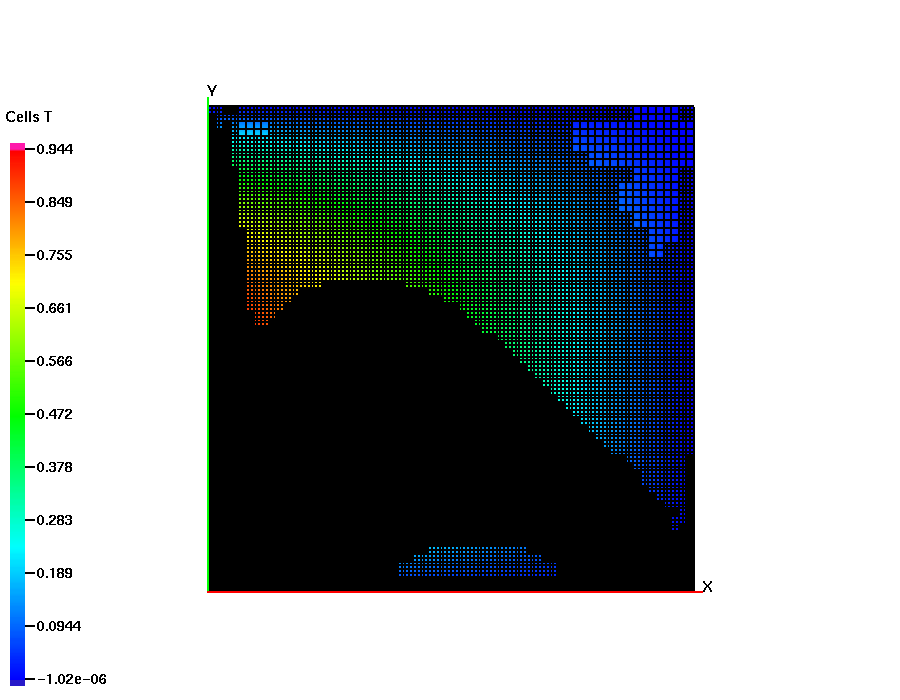
\includegraphics[width=.3\textwidth]{adjoint_grid2}
\end{center}


\end{frame}

%===============================================================================
% NEW SLIDE
%===============================================================================
\begin{frame}
\frametitle{Manufactured Solution Example}
\begin{columns}
\begin{column}{.55\textwidth}
\begin{block}{Adjoint-based Parameter Sensitivity}
\begin{itemize}
\item Convergence to analytic sensitivity plateaus at $2\%$ relative
error in {\bf every} refinement strategy
\item Finite differenced partial derivatives not responsible
\item Manufactured solution allowed sensitivity subcomponent
comparison to analytic solutions
\item Sign errors in \libMesh{} parameter sensitivity method
\end{itemize}
\end{block}
\end{column}
\begin{column}{.45\textwidth}
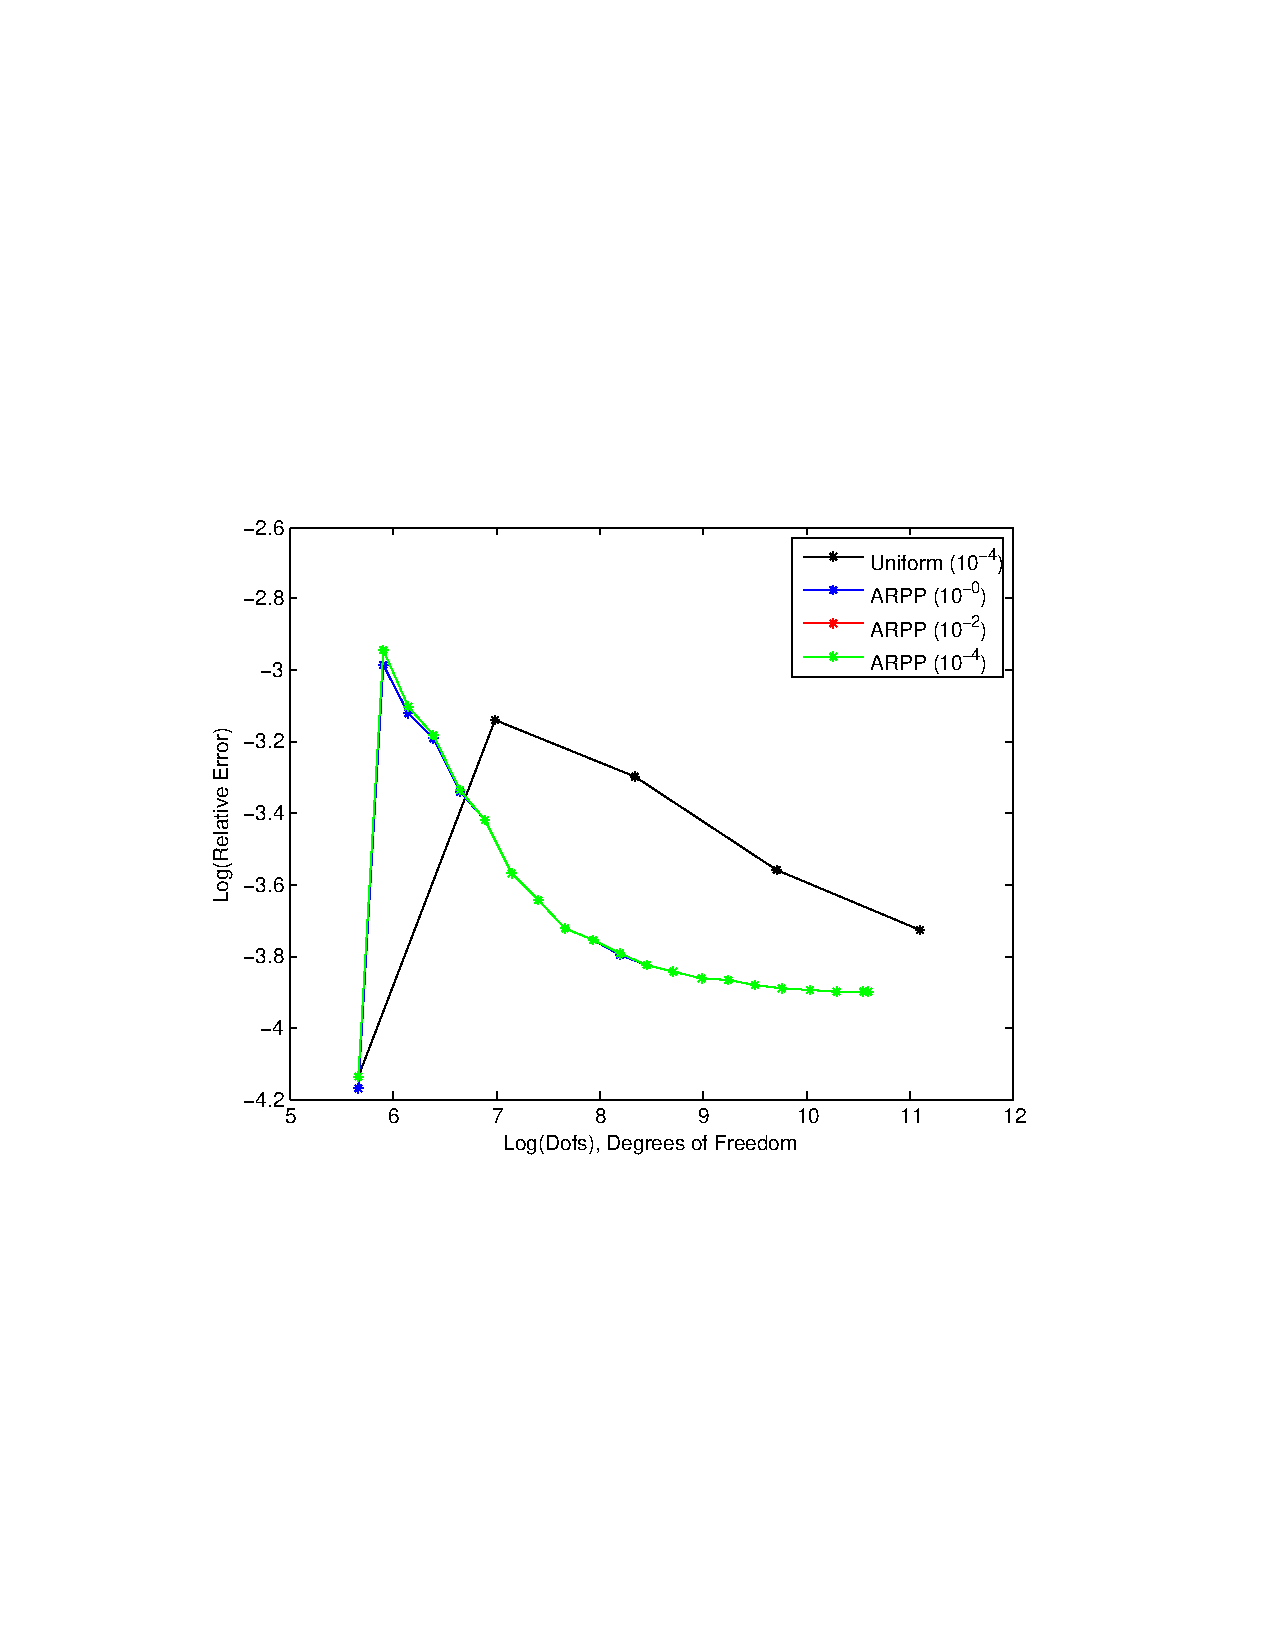
\includegraphics[width=\textwidth]{sensitivity_plateau_FD_test}
\end{column}
\end{columns}

\end{frame}

%===============================================================================
% NEW SLIDE
%===============================================================================
\begin{frame}
\frametitle{Manufactured Solution Example}
\begin{columns}
\begin{column}{.45\textwidth}
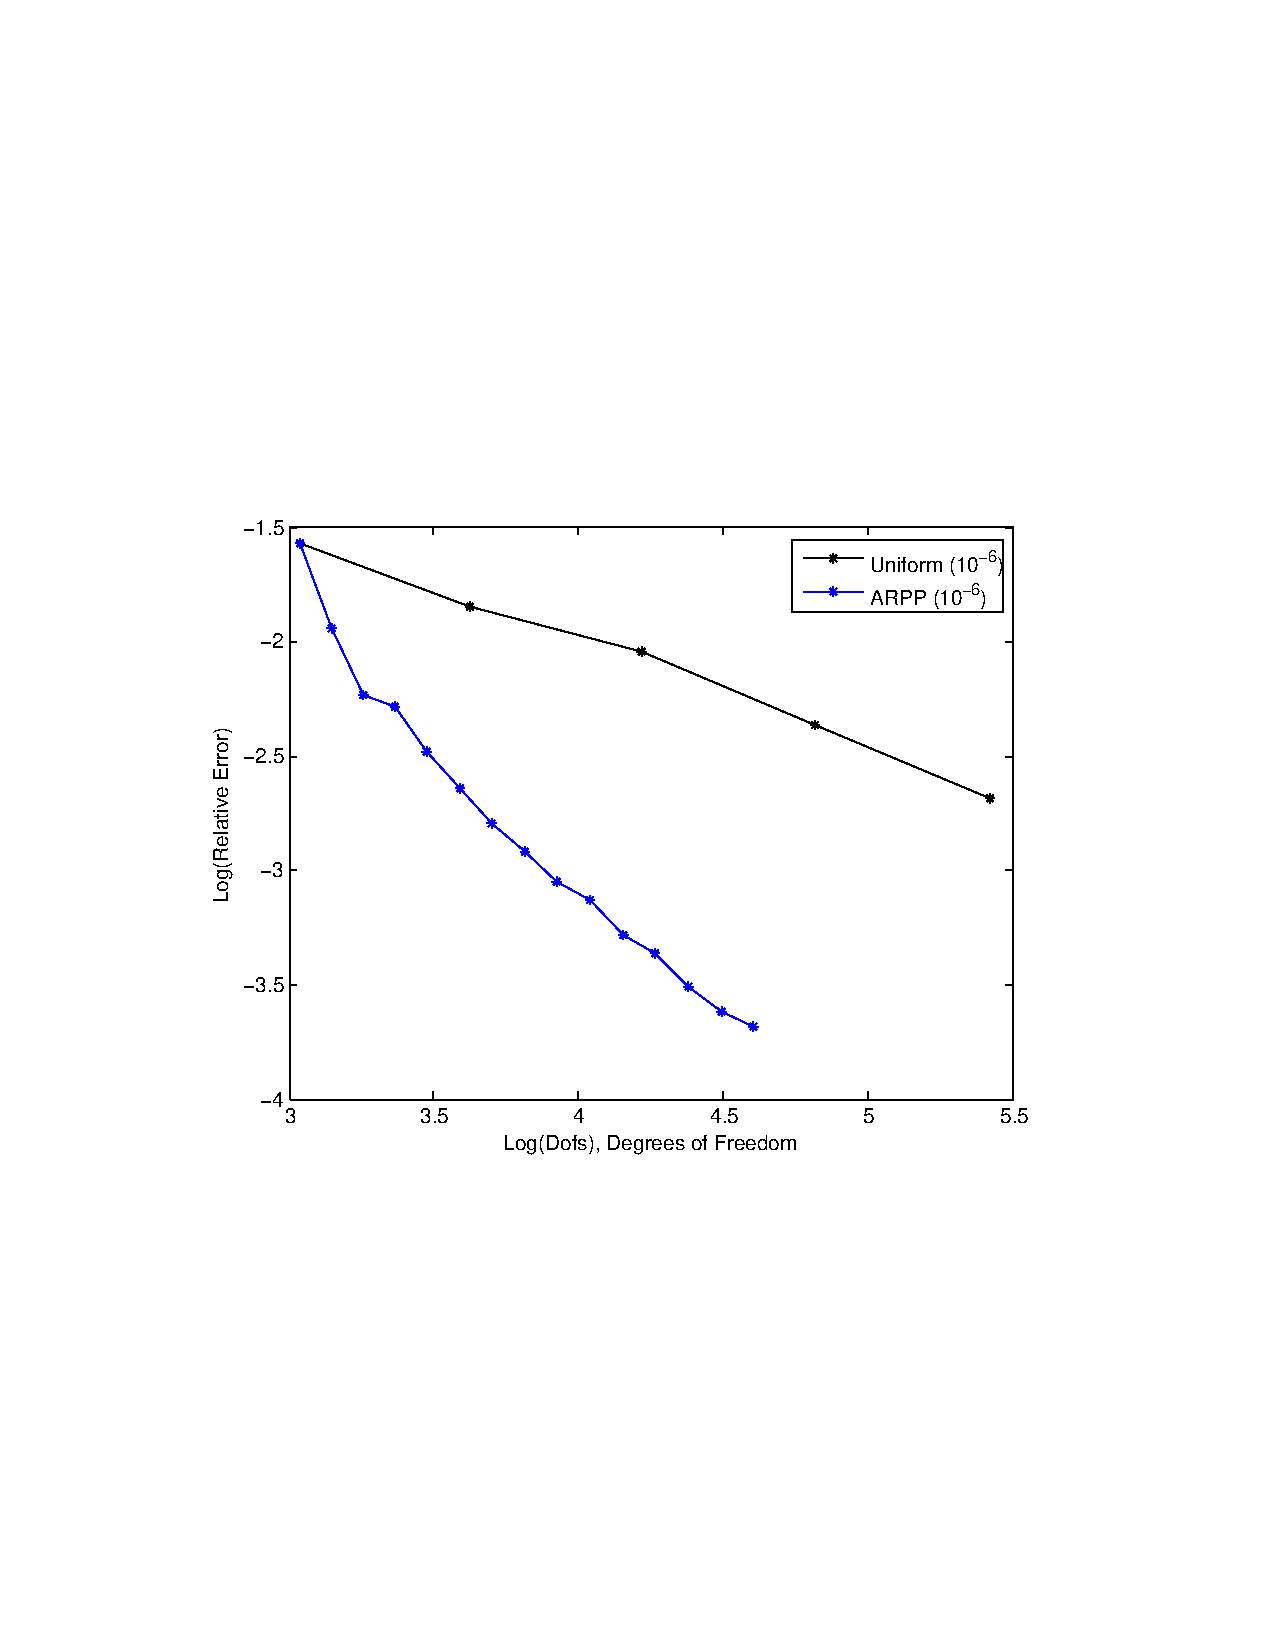
\includegraphics[width=\textwidth]{sensitivity_convergence}
\end{column}
\begin{column}{.55\textwidth}
\begin{block}{Adjoint-based Parameter Sensitivity}
\begin{itemize}
\item ``Off by 100\%'' error remaining in one subterm of equations
\item Switch to $u''=f$, 1D quadratic solutions, manufactured residual test
\item Identified bug in repeated \texttt{adjoint\_solve} rhs assembly
\item Returned to manufactured solution benchmark: now converges to
true solution
\end{itemize}
\end{block}
\end{column}
\end{columns}

\end{frame}


%===============================================================================
% NEW SLIDE
%===============================================================================
\begin{frame}
\frametitle{Manufactured Solution Issues}
\begin{block}{Compressible Inviscid Perfect Gas Flow}

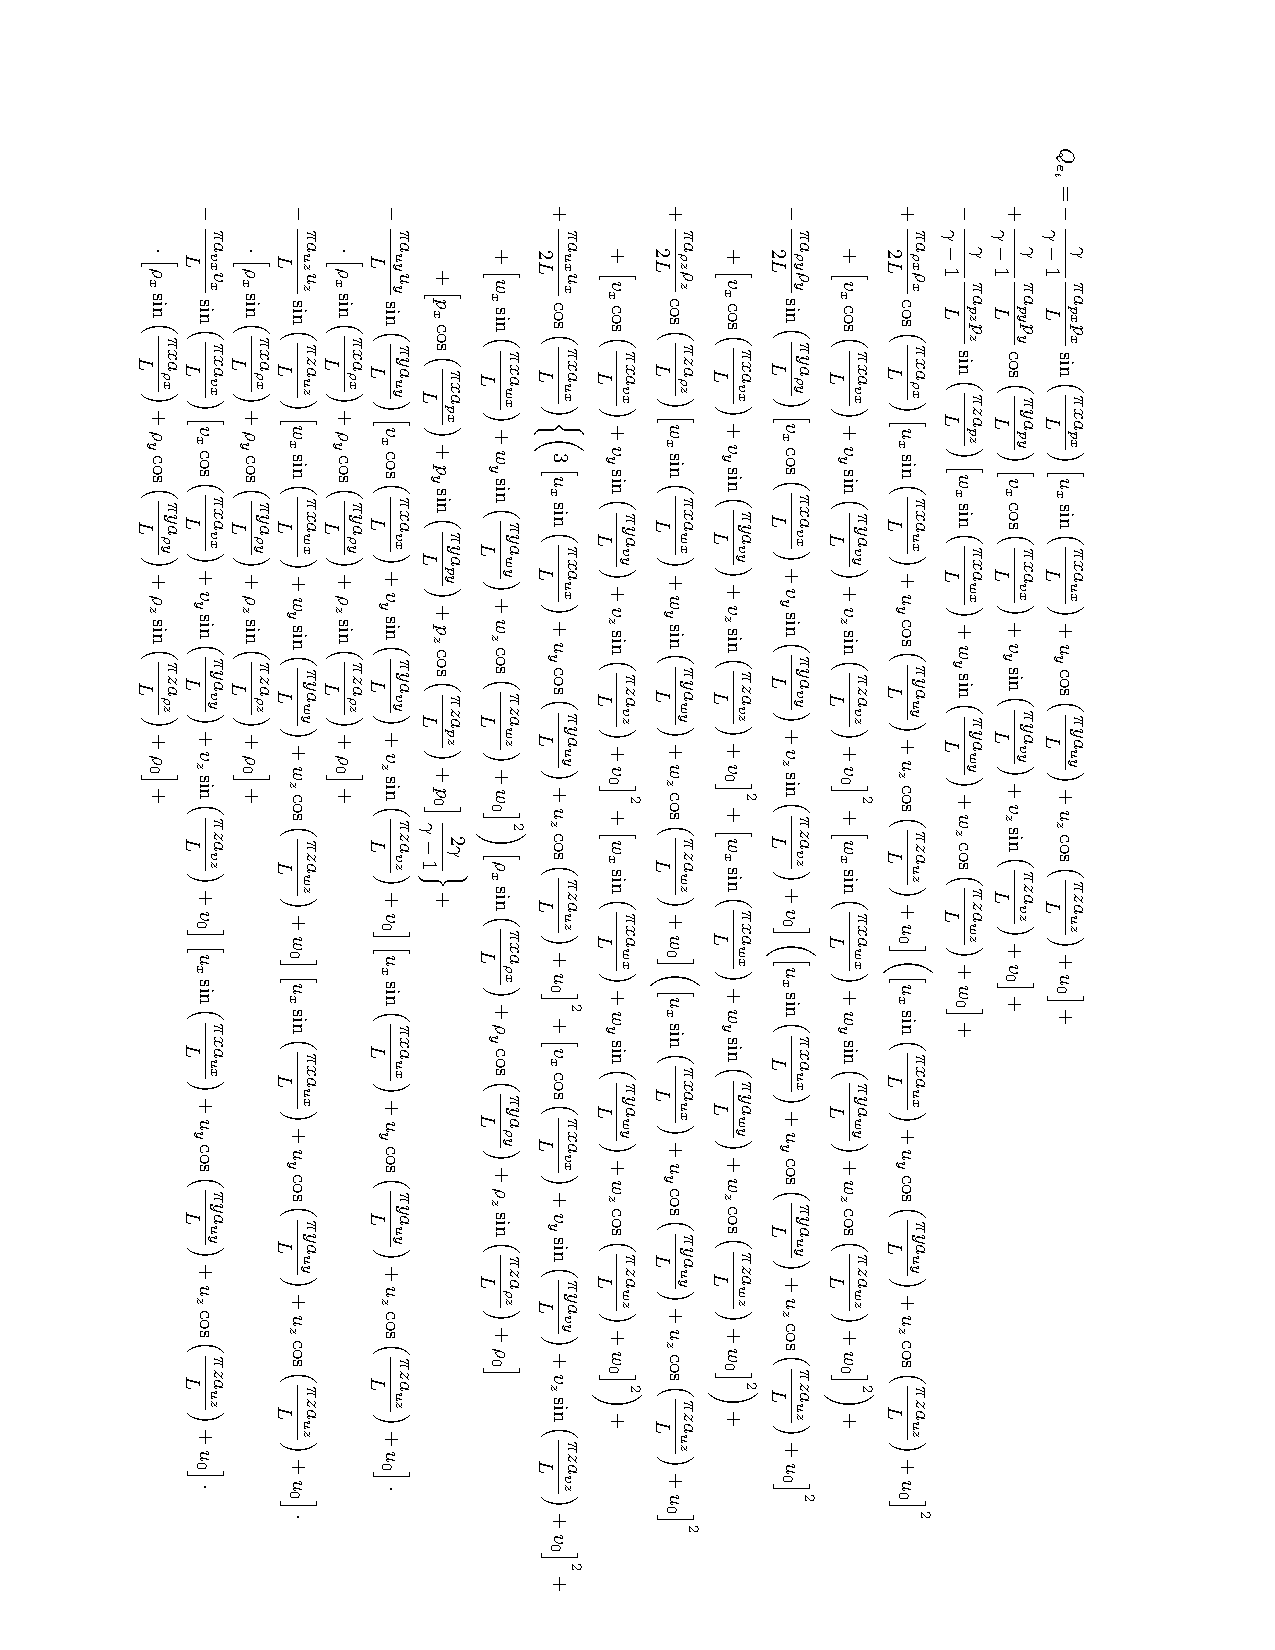
\includegraphics[height=.45\textwidth,angle=90]{energy_equation_forcing1}
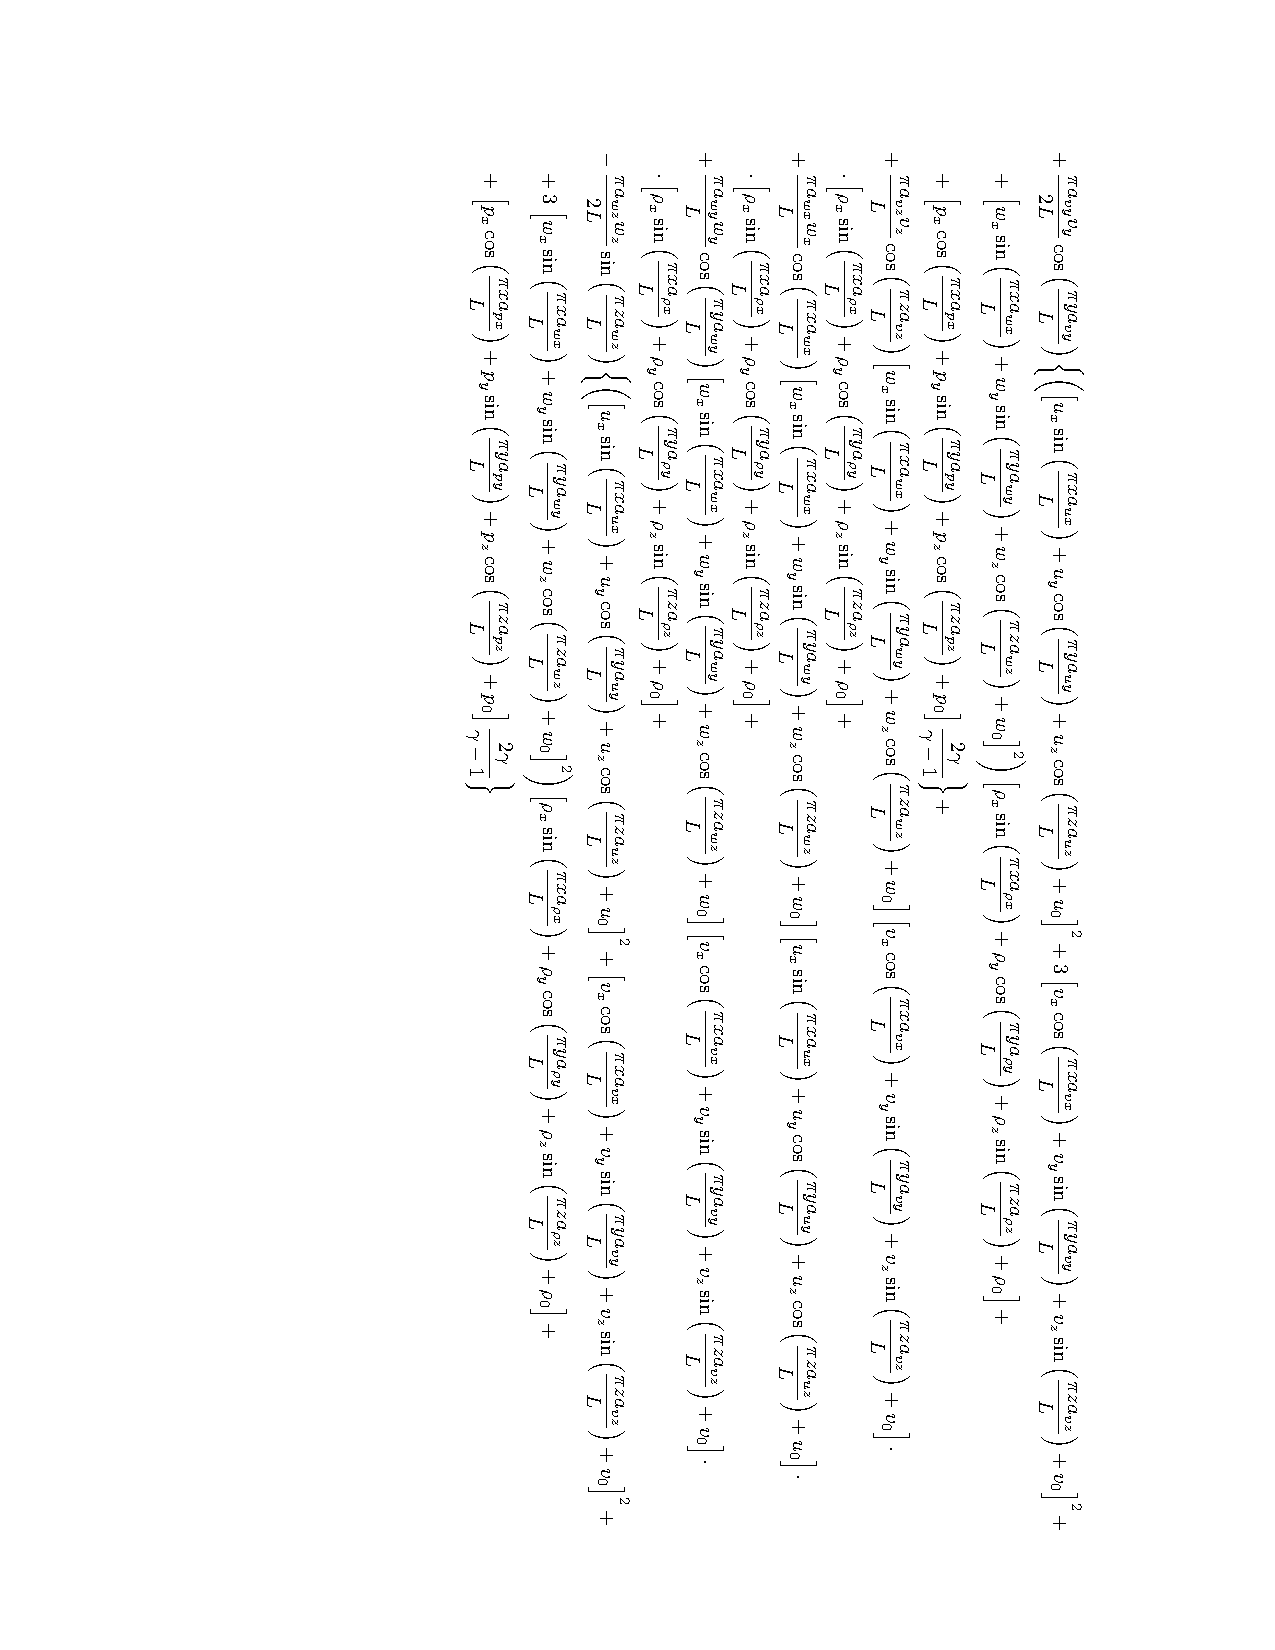
\includegraphics[height=.45\textwidth,angle=90]{energy_equation_forcing2}

\end{block}

\begin{itemize}
\item Use Maple, Mathematica, automatic differentiation
\item Manufactured Analytic Solution Abstraction library:
      \url{https://manufactured-solutions.github.io/MASA/}
\end{itemize}

\end{frame}

\subsection{Application Verification}

%===============================================================================
% NEW SLIDE
%===============================================================================
\begin{frame}
\frametitle{Code-to-Code, Code-to-Experiment}
\begin{itemize}
  \item Validation: Solving the right equations
  \item Verification: Solving the equations right
\end{itemize}
\begin{columns}
\begin{column}{.7\textwidth}
\begin{block}{``Lumped'' Verification + Validation}
\begin{itemize}
\item ``Error'' can be indistinguishable from non-errors, giving false
  positives
\begin{itemize}
\item Different experimental assumptions
\item Different physical models
\item Different mathematical formulations
\item Different numerical discretizations
\end{itemize}
\item Error contributions can \emph{cancel} in test scenarios, giving
  false negatives
\item Uncaught error terms can \emph{extrapolate} in a use case
\end{itemize}
\end{block}
\end{column}
\begin{column}{.3\textwidth}
\begin{center}
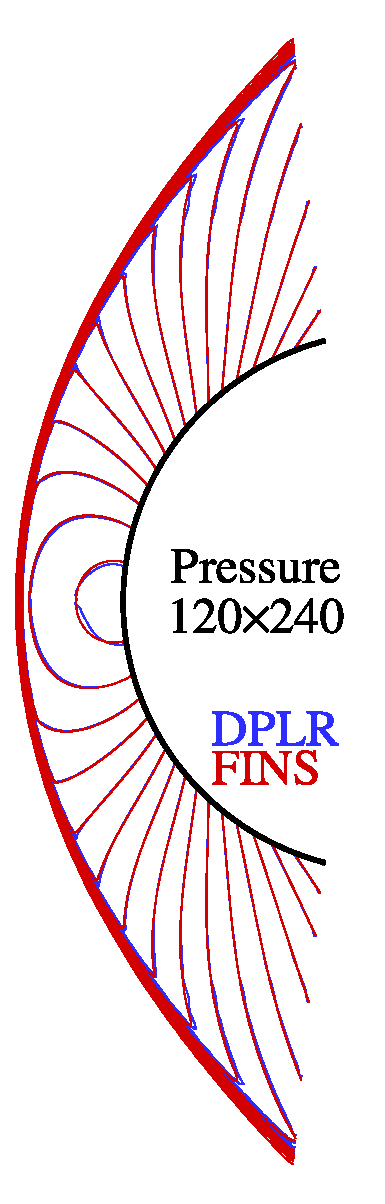
\includegraphics[width=.5\textwidth]{dplr_fins}
\end{center}
\end{column}
\end{columns}

\end{frame}

%===============================================================================
% NEW SLIDE
%===============================================================================
\begin{frame}
\frametitle{A Priori Asymptotic Convergence Rates}
\begin{block}{Biharmonic Problem, Manufactured Solution}
\begin{itemize}
\item $\Delta^2 \V{u} = \V{f}$
\item $C^1$ Macroelement bases
\end{itemize}
\end{block}

\begin{columns}
\begin{column}{.5\textwidth}
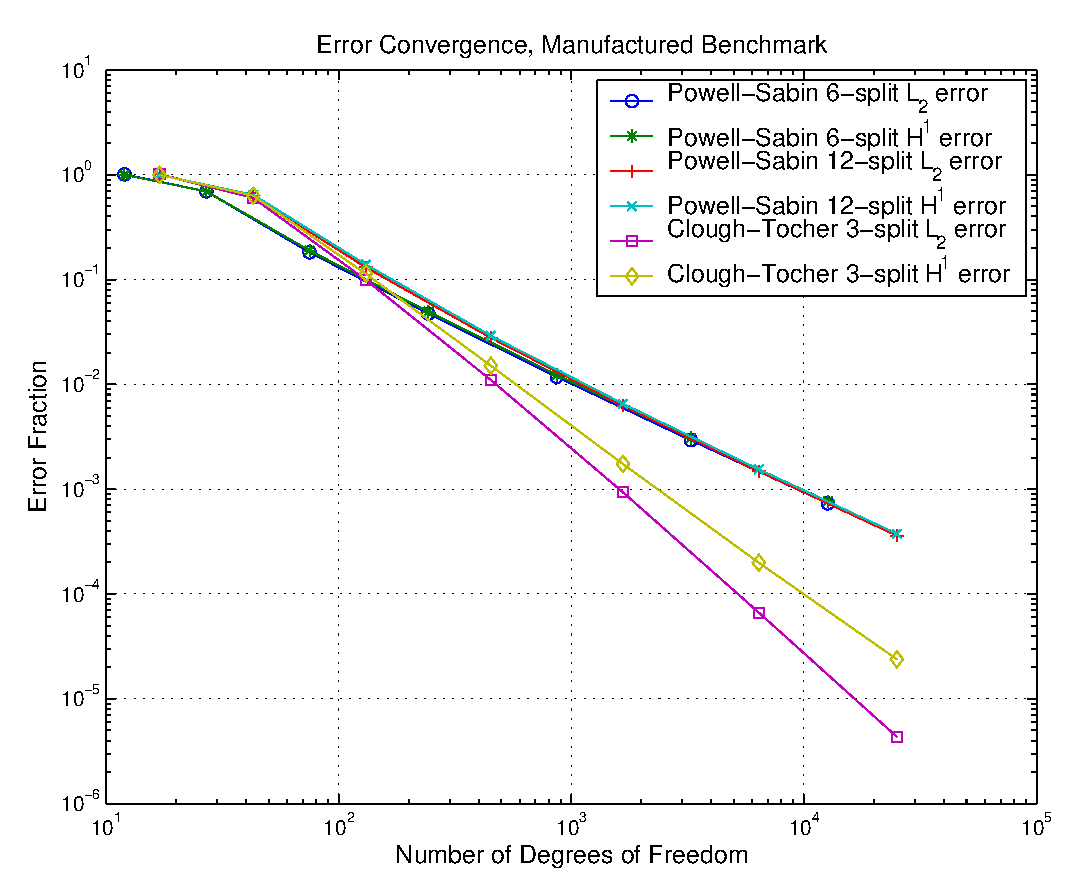
\includegraphics[width=\textwidth]{macroelement}
\end{column}
\begin{column}{.5\textwidth}
\begin{block}{Verification Example}
\begin{itemize}
\item Code verification failures - bugs in basis transformations
\item Solution verification ``failure'' - higher order Nitsche lift
fails for $L_2$ error with quadratic elements for fourth order problems
\end{itemize}
\end{block}
\end{column}
\end{columns}

\end{frame}

%===============================================================================
% NEW SLIDE
%===============================================================================
\begin{frame}
\frametitle{Asymptotic Convergence Rate Examples}
\begin{block}{Cahn-Hilliard Phase Evolution}
\begin{center}
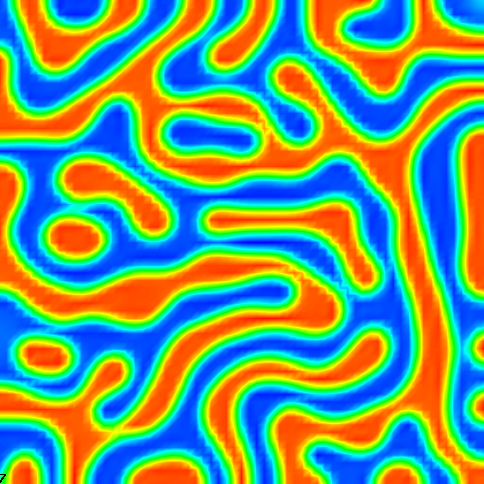
\includegraphics[width=.25\textwidth]{chem-0250}
\;\;\;

\includegraphics[width=.25\textwidth]{chem-0500}
\;\;\;

\includegraphics[width=.25\textwidth]{chem-1000}
\end{center}
\end{block}

\begin{columns}
\begin{column}{.4\textwidth}
\begin{center}
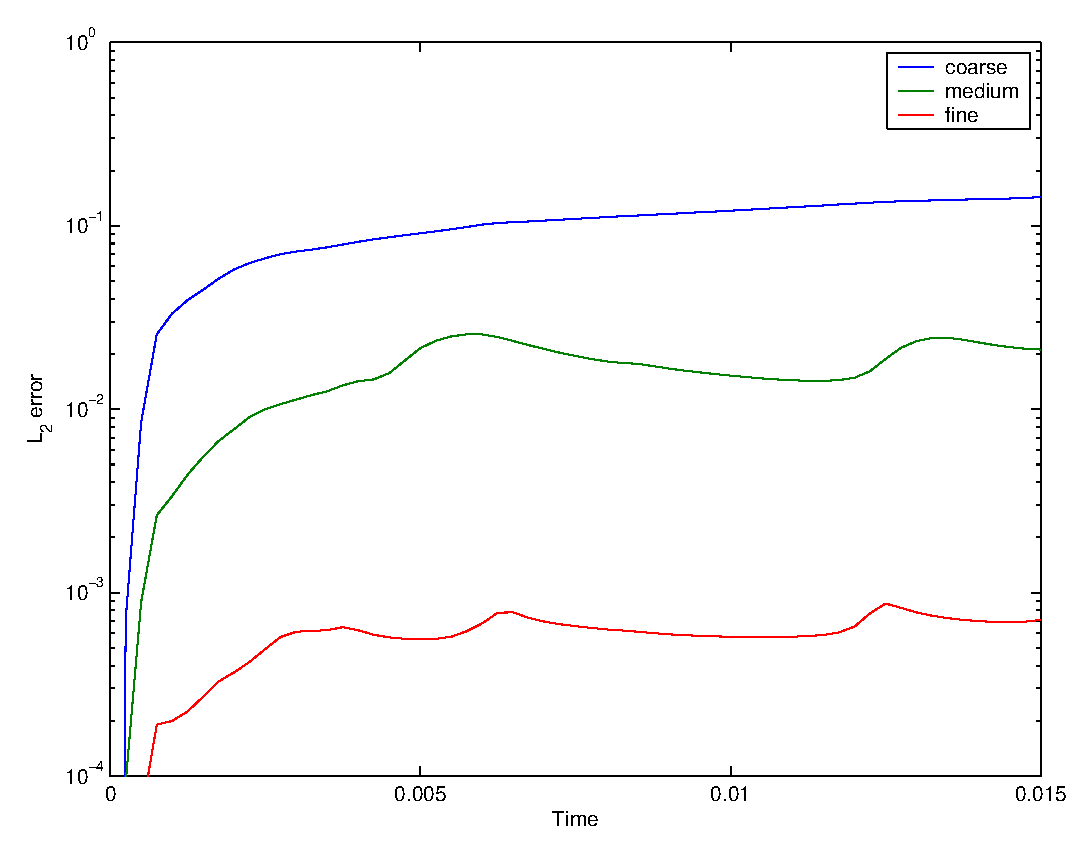
\includegraphics[width=.8\textwidth]{cherror}
\end{center}
\end{column}
\begin{column}{.6\textwidth}
Gives some confidence in even highly nonlinear, transient, stochastic problems
\end{column}
\end{columns}

\end{frame}

